\section{RCRRT  Class Reference}
\label{classRCRRT}\index{RCRRT@{RCRRT}}
Resolution Complete Rapidly-Exploring Random Trees , by Peng Cheng and Steven M. La\-Valle, submitted to 2002 IEEE International Conference on Robotics and Automation. Techniques applied to improve the performance: (1) Combining systematic search with random search such that it has both the completeness of the systematic search and fast searching of the random search. (2) Constraint violation tendency to avoid obstacles This basic planner is used to do the experiment with dynamic car model in the virtual town. The rolling effect of the car and the nonlinear tire model are considered in the model. 


{\tt \#include $<$rcrrt.h$>$}

Inheritance diagram for RCRRT::\begin{figure}[H]
\begin{center}
\leavevmode
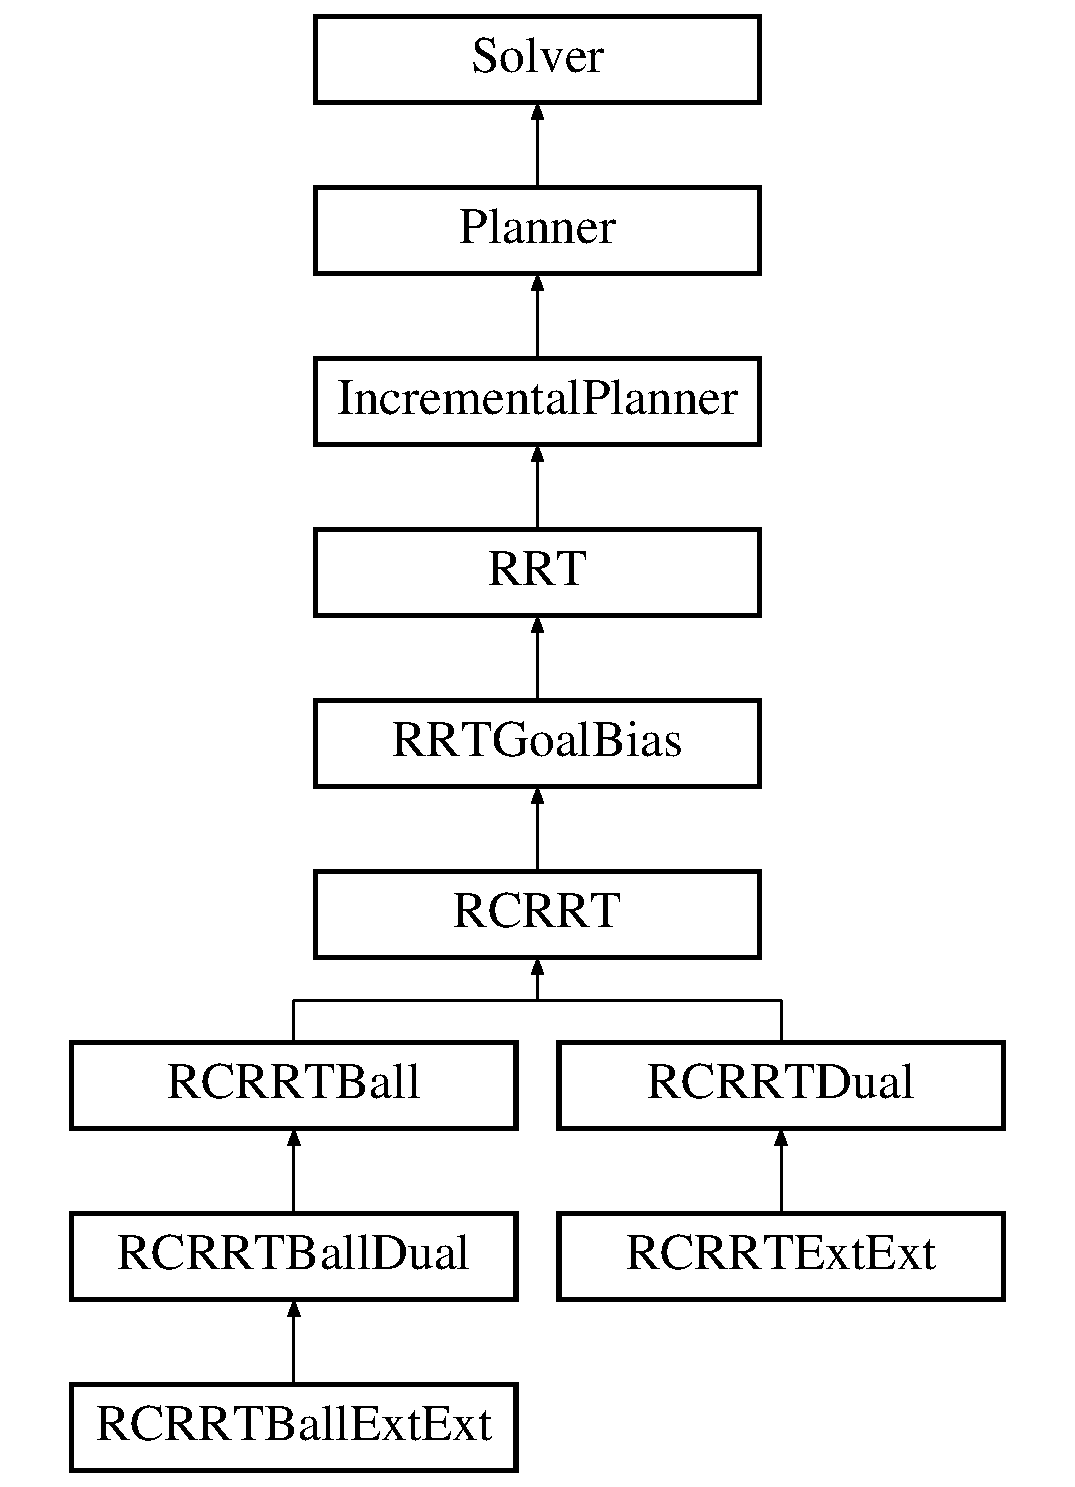
\includegraphics[height=9cm]{classRCRRT}
\end{center}
\end{figure}
\subsection*{Public Methods}
\begin{CompactItemize}
\item 
bool {\bf Is\-Node\-Expanded} ({\bf MSLNode} $\ast${\bf x}, double \&biasvalue, bool forward)
\begin{CompactList}\small\item\em Check if this node has been explored (all inputs are expanded) and return the collision tendency information Used in Select\-Node function.\item\end{CompactList}\item 
virtual bool {\bf Is\-Input\-Applied} (const int \&inputindex, const {\bf MSLVector} \&expolreinfo)
\begin{CompactList}\small\item\em Check the ith input is failed or not Used in Select\-Input function.\item\end{CompactList}\item 
virtual void {\bf Back\-Ward\-Bias\-Set} ({\bf MSLNode} $\ast$n, {\bf MSLTree} $\ast$t)
\begin{CompactList}\small\item\em back ward along the tree to set the bias value.\item\end{CompactList}\item 
double {\bf Bias\-Value} (int backstep)
\begin{CompactList}\small\item\em bias value function,.\item\end{CompactList}\item 
{\bf RCRRT} ({\bf Problem} $\ast$problem)
\item 
virtual {\bf $\sim$RCRRT} ()
\item 
virtual {\bf MSLNode} $\ast$ {\bf Select\-Node} (const {\bf MSLVector} \&{\bf x}, {\bf MSLTree} $\ast$t, bool forward)
\begin{CompactList}\small\item\em Select the nearestneighbor node according to given metric !!!!!!!!!!!!!!!!!!!!!!!!!!!!!!!!!!! This function is metric dependent !!!!!!!!!!!!!!!!!!!!!!!!!!!!!!!!!!! Choose the nestest neighbor in the search structure If all nodes are explored, return (NULL) node If there exist unexpanded nodes (1) return the closest node with probability equal collisiontendency (2) or, return the closed node when (2) return nothing.\item\end{CompactList}\item 
virtual bool {\bf Extend} (const {\bf MSLVector} \&{\bf x}, {\bf MSLTree} $\ast$t, {\bf MSLNode} $\ast$\&nn, bool forward)
\begin{CompactList}\small\item\em Extend the nearest node to the random state return true: a new node is generated return false: 1. all the successors of the chosen node are in collision 2. no nearest node is chosen because all of them are explored.\item\end{CompactList}\item 
virtual {\bf MSLVector} {\bf Select\-Input} ({\bf MSLNode} $\ast$n1, const {\bf MSLVector} \&x2, {\bf MSLVector} \&nx\_\-best, bool \&success, bool forward)
\begin{CompactList}\small\item\em The first parameter is node because the node will be used in the function, xu\_\-new is the new value for the uncontrolled state.\item\end{CompactList}\item 
virtual bool {\bf Connect} (const {\bf MSLVector} \&{\bf x}, {\bf MSLTree} $\ast$t, {\bf MSLNode} $\ast$\&nn, bool forward)
\begin{CompactList}\small\item\em method to increase the extending time because the more time the RCRRT extend in each step, more quickly the overall information of state space is gotten.\item\end{CompactList}\item 
virtual bool {\bf Plan} ()
\begin{CompactList}\small\item\em Attempt to solve an Initial-Goal query by growing an {\bf RRT} {\rm (p.\,\pageref{classRRT})}.\item\end{CompactList}\end{CompactItemize}
\subsection*{Public Attributes}
\begin{CompactItemize}
\item 
int {\bf inputnum}
\begin{CompactList}\small\item\em the number of the inputs.\item\end{CompactList}\item 
list$<$ {\bf MSLVector} $>$ {\bf inputset}
\begin{CompactList}\small\item\em input set.\item\end{CompactList}\item 
bool {\bf issolutionexist}
\begin{CompactList}\small\item\em true, solution possibly exists; false, solution does not exist.\item\end{CompactList}\item 
{\bf MSLVector} {\bf initexploreinfo}
\begin{CompactList}\small\item\em Initial exploration information initialized with 0.\item\end{CompactList}\item 
double {\bf initcoltend}
\begin{CompactList}\small\item\em Initial collision tendency.\item\end{CompactList}\end{CompactItemize}


\subsection{Detailed Description}
Resolution Complete Rapidly-Exploring Random Trees , by Peng Cheng and Steven M. La\-Valle, submitted to 2002 IEEE International Conference on Robotics and Automation. Techniques applied to improve the performance: (1) Combining systematic search with random search such that it has both the completeness of the systematic search and fast searching of the random search. (2) Constraint violation tendency to avoid obstacles This basic planner is used to do the experiment with dynamic car model in the virtual town. The rolling effect of the car and the nonlinear tire model are considered in the model.



\subsection{Constructor \& Destructor Documentation}
\index{RCRRT@{RCRRT}!RCRRT@{RCRRT}}
\index{RCRRT@{RCRRT}!RCRRT@{RCRRT}}
\subsubsection{\setlength{\rightskip}{0pt plus 5cm}RCRRT::RCRRT ({\bf Problem} $\ast$ {\em problem})}\label{classRCRRT_a4}


\index{RCRRT@{RCRRT}!~RCRRT@{$\sim$RCRRT}}
\index{~RCRRT@{$\sim$RCRRT}!RCRRT@{RCRRT}}
\subsubsection{\setlength{\rightskip}{0pt plus 5cm}virtual RCRRT::$\sim$RCRRT ()\hspace{0.3cm}{\tt  [inline, virtual]}}\label{classRCRRT_a5}




\subsection{Member Function Documentation}
\index{RCRRT@{RCRRT}!BackWardBiasSet@{BackWardBiasSet}}
\index{BackWardBiasSet@{BackWardBiasSet}!RCRRT@{RCRRT}}
\subsubsection{\setlength{\rightskip}{0pt plus 5cm}void RCRRT::Back\-Ward\-Bias\-Set ({\bf MSLNode} $\ast$ {\em n}, {\bf MSLTree} $\ast$ {\em t})\hspace{0.3cm}{\tt  [virtual]}}\label{classRCRRT_a2}


back ward along the tree to set the bias value.

\index{RCRRT@{RCRRT}!BiasValue@{BiasValue}}
\index{BiasValue@{BiasValue}!RCRRT@{RCRRT}}
\subsubsection{\setlength{\rightskip}{0pt plus 5cm}double RCRRT::Bias\-Value (int {\em backstep})}\label{classRCRRT_a3}


bias value function,.

\index{RCRRT@{RCRRT}!Connect@{Connect}}
\index{Connect@{Connect}!RCRRT@{RCRRT}}
\subsubsection{\setlength{\rightskip}{0pt plus 5cm}bool RCRRT::Connect (const {\bf MSLVector} \& {\em x}, {\bf MSLTree} $\ast$ {\em t}, {\bf MSLNode} $\ast$\& {\em nn}, bool {\em forward})\hspace{0.3cm}{\tt  [virtual]}}\label{classRCRRT_a9}


method to increase the extending time because the more time the RCRRT extend in each step, more quickly the overall information of state space is gotten.



Reimplemented from {\bf RRT} {\rm (p.\,\pageref{classRRT_b3})}.

Reimplemented in {\bf RCRRTBall} {\rm (p.\,\pageref{classRCRRTBall_a4})}.\index{RCRRT@{RCRRT}!Extend@{Extend}}
\index{Extend@{Extend}!RCRRT@{RCRRT}}
\subsubsection{\setlength{\rightskip}{0pt plus 5cm}bool RCRRT::Extend (const {\bf MSLVector} \& {\em x}, {\bf MSLTree} $\ast$ {\em t}, {\bf MSLNode} $\ast$\& {\em nn}, bool {\em forward})\hspace{0.3cm}{\tt  [virtual]}}\label{classRCRRT_a7}


Extend the nearest node to the random state return true: a new node is generated return false: 1. all the successors of the chosen node are in collision 2. no nearest node is chosen because all of them are explored.



Reimplemented from {\bf RRT} {\rm (p.\,\pageref{classRRT_b2})}.

Reimplemented in {\bf RCRRTBall} {\rm (p.\,\pageref{classRCRRTBall_a3})}.\index{RCRRT@{RCRRT}!IsInputApplied@{IsInputApplied}}
\index{IsInputApplied@{IsInputApplied}!RCRRT@{RCRRT}}
\subsubsection{\setlength{\rightskip}{0pt plus 5cm}bool RCRRT::Is\-Input\-Applied (const int \& {\em inputindex}, const {\bf MSLVector} \& {\em expolreinfo})\hspace{0.3cm}{\tt  [virtual]}}\label{classRCRRT_a1}


Check the ith input is failed or not Used in Select\-Input function.

\index{RCRRT@{RCRRT}!IsNodeExpanded@{IsNodeExpanded}}
\index{IsNodeExpanded@{IsNodeExpanded}!RCRRT@{RCRRT}}
\subsubsection{\setlength{\rightskip}{0pt plus 5cm}bool RCRRT::Is\-Node\-Expanded ({\bf MSLNode} $\ast$ {\em x}, double \& {\em biasvalue}, bool {\em forward})}\label{classRCRRT_a0}


Check if this node has been explored (all inputs are expanded) and return the collision tendency information Used in Select\-Node function.

\index{RCRRT@{RCRRT}!Plan@{Plan}}
\index{Plan@{Plan}!RCRRT@{RCRRT}}
\subsubsection{\setlength{\rightskip}{0pt plus 5cm}bool RCRRT::Plan ()\hspace{0.3cm}{\tt  [virtual]}}\label{classRCRRT_a10}


Attempt to solve an Initial-Goal query by growing an {\bf RRT} {\rm (p.\,\pageref{classRRT})}.



Reimplemented from {\bf RRT} {\rm (p.\,\pageref{classRRT_a3})}.

Reimplemented in {\bf RCRRTDual} {\rm (p.\,\pageref{classRCRRTDual_a2})}.\index{RCRRT@{RCRRT}!SelectInput@{SelectInput}}
\index{SelectInput@{SelectInput}!RCRRT@{RCRRT}}
\subsubsection{\setlength{\rightskip}{0pt plus 5cm}{\bf MSLVector} RCRRT::Select\-Input ({\bf MSLNode} $\ast$ {\em n1}, const {\bf MSLVector} \& {\em x2}, {\bf MSLVector} \& {\em nx\_\-best}, bool \& {\em success}, bool {\em forward})\hspace{0.3cm}{\tt  [virtual]}}\label{classRCRRT_a8}


The first parameter is node because the node will be used in the function, xu\_\-new is the new value for the uncontrolled state.

\index{RCRRT@{RCRRT}!SelectNode@{SelectNode}}
\index{SelectNode@{SelectNode}!RCRRT@{RCRRT}}
\subsubsection{\setlength{\rightskip}{0pt plus 5cm}{\bf MSLNode} $\ast$ RCRRT::Select\-Node (const {\bf MSLVector} \& {\em x}, {\bf MSLTree} $\ast$ {\em t}, bool {\em forward})\hspace{0.3cm}{\tt  [virtual]}}\label{classRCRRT_a6}


Select the nearestneighbor node according to given metric !!!!!!!!!!!!!!!!!!!!!!!!!!!!!!!!!!! This function is metric dependent !!!!!!!!!!!!!!!!!!!!!!!!!!!!!!!!!!! Choose the nestest neighbor in the search structure If all nodes are explored, return (NULL) node If there exist unexpanded nodes (1) return the closest node with probability equal collisiontendency (2) or, return the closed node when (2) return nothing.



Reimplemented from {\bf RRT} {\rm (p.\,\pageref{classRRT_b1})}.

Reimplemented in {\bf RCRRTBall} {\rm (p.\,\pageref{classRCRRTBall_a2})}.

\subsection{Member Data Documentation}
\index{RCRRT@{RCRRT}!initcoltend@{initcoltend}}
\index{initcoltend@{initcoltend}!RCRRT@{RCRRT}}
\subsubsection{\setlength{\rightskip}{0pt plus 5cm}double RCRRT::initcoltend}\label{classRCRRT_m4}


Initial collision tendency.

\index{RCRRT@{RCRRT}!initexploreinfo@{initexploreinfo}}
\index{initexploreinfo@{initexploreinfo}!RCRRT@{RCRRT}}
\subsubsection{\setlength{\rightskip}{0pt plus 5cm}{\bf MSLVector} RCRRT::initexploreinfo}\label{classRCRRT_m3}


Initial exploration information initialized with 0.

\index{RCRRT@{RCRRT}!inputnum@{inputnum}}
\index{inputnum@{inputnum}!RCRRT@{RCRRT}}
\subsubsection{\setlength{\rightskip}{0pt plus 5cm}int RCRRT::inputnum}\label{classRCRRT_m0}


the number of the inputs.

\index{RCRRT@{RCRRT}!inputset@{inputset}}
\index{inputset@{inputset}!RCRRT@{RCRRT}}
\subsubsection{\setlength{\rightskip}{0pt plus 5cm}list$<${\bf MSLVector}$>$ RCRRT::inputset}\label{classRCRRT_m1}


input set.

\index{RCRRT@{RCRRT}!issolutionexist@{issolutionexist}}
\index{issolutionexist@{issolutionexist}!RCRRT@{RCRRT}}
\subsubsection{\setlength{\rightskip}{0pt plus 5cm}bool RCRRT::issolutionexist}\label{classRCRRT_m2}


true, solution possibly exists; false, solution does not exist.



The documentation for this class was generated from the following files:\begin{CompactItemize}
\item 
{\bf rcrrt.h}\item 
{\bf rcrrt.C}\end{CompactItemize}
